\documentclass[10pt]{beamer}

\usepackage{polyglossia}
\usepackage{csquotes}
\usepackage{datetime}
\usepackage{fontspec}
\usepackage{microtype}
\usepackage{color}
\usepackage{url}
\usepackage{hyperref}
\usepackage{amsfonts}
\usepackage{amsmath}
\usepackage{amsthm}
\usepackage{subcaption}
\usepackage[backend=biber,style=iso-authoryear,sortlocale=en_US,autolang=other,bibencoding=UTF8]{biblatex}
\usepackage{booktabs}
\usepackage{graphics}
\usepackage{pifont}
\usepackage{ulem}
\usepackage{tikz}

%\addbibresource{zotero.bib}

\setdefaultlanguage{english}
\setmainfont{TeX Gyre Termes}
\usetheme{Boadilla}
\usecolortheme{crane}
\setbeamertemplate{title page}[default][rounded=true,shadow=false]
\setbeamertemplate{section in toc}[ball unnumbered]
\setbeamertemplate{bibliography item}{}

\hypersetup{
	pdfencoding=auto,
	unicode=true,
	citecolor=green,
	filecolor=blue,
	linkcolor=red,
	urlcolor=blue
}

\makeatletter
\newcommand*{\currentSection}{\@currentlabelname}
\makeatother

\newcommand{\mathmat}{\ensuremath{\mathbf}}

\title[DDny KM FJFI 2021]
{
	Graph Coarsening Can Increase Learning Efficiency
}

\newdate{presentation}{19}{11}{2021}
\date[November 2021]{\displaydate{presentation}}

\author[Marek Dědič]
{
	Marek~Dědič
}

\institute[Cisco]{}

% TOC
%\AtBeginSection[]{
	%\begin{frame}{\currentSection}
		%\tableofcontents[currentsection]
	%\end{frame}
%}

% Title card
\AtBeginSection[]{
  \begin{frame}
  \vfill
  \centering
  \begin{beamercolorbox}[sep=8pt,center,shadow=true,rounded=true]{title}
    \usebeamerfont{title}\insertsectionhead\par%
  \end{beamercolorbox}
  \vfill
  \end{frame}
}

\begin{document}

\begin{frame}
  \titlepage
\end{frame}

% Body

\section{Subgraph isomorphisms}

\begin{frame}{Malware moving infrastructure}
	\begin{itemize}
	      \item Malware in the \enquote{wild} sometimes ceases using a particular piece of infrastructure and moves to a different one
	      \item Currently, we have no way to detect this
	      \item We would like to detect the infrastructure going dark and flag the CT as probably having new infra
	      \item Ideally, as the next step, we would like to predict the new infrastructure the particular CT might use and suggest it for manual review
	      \item We have some theoretical background that should help with this - the notion of subgraph isomorphisms
	\end{itemize}
\end{frame}

\begin{frame}{Malware moving infrastructure}
	\begin{figure}
		\centering
		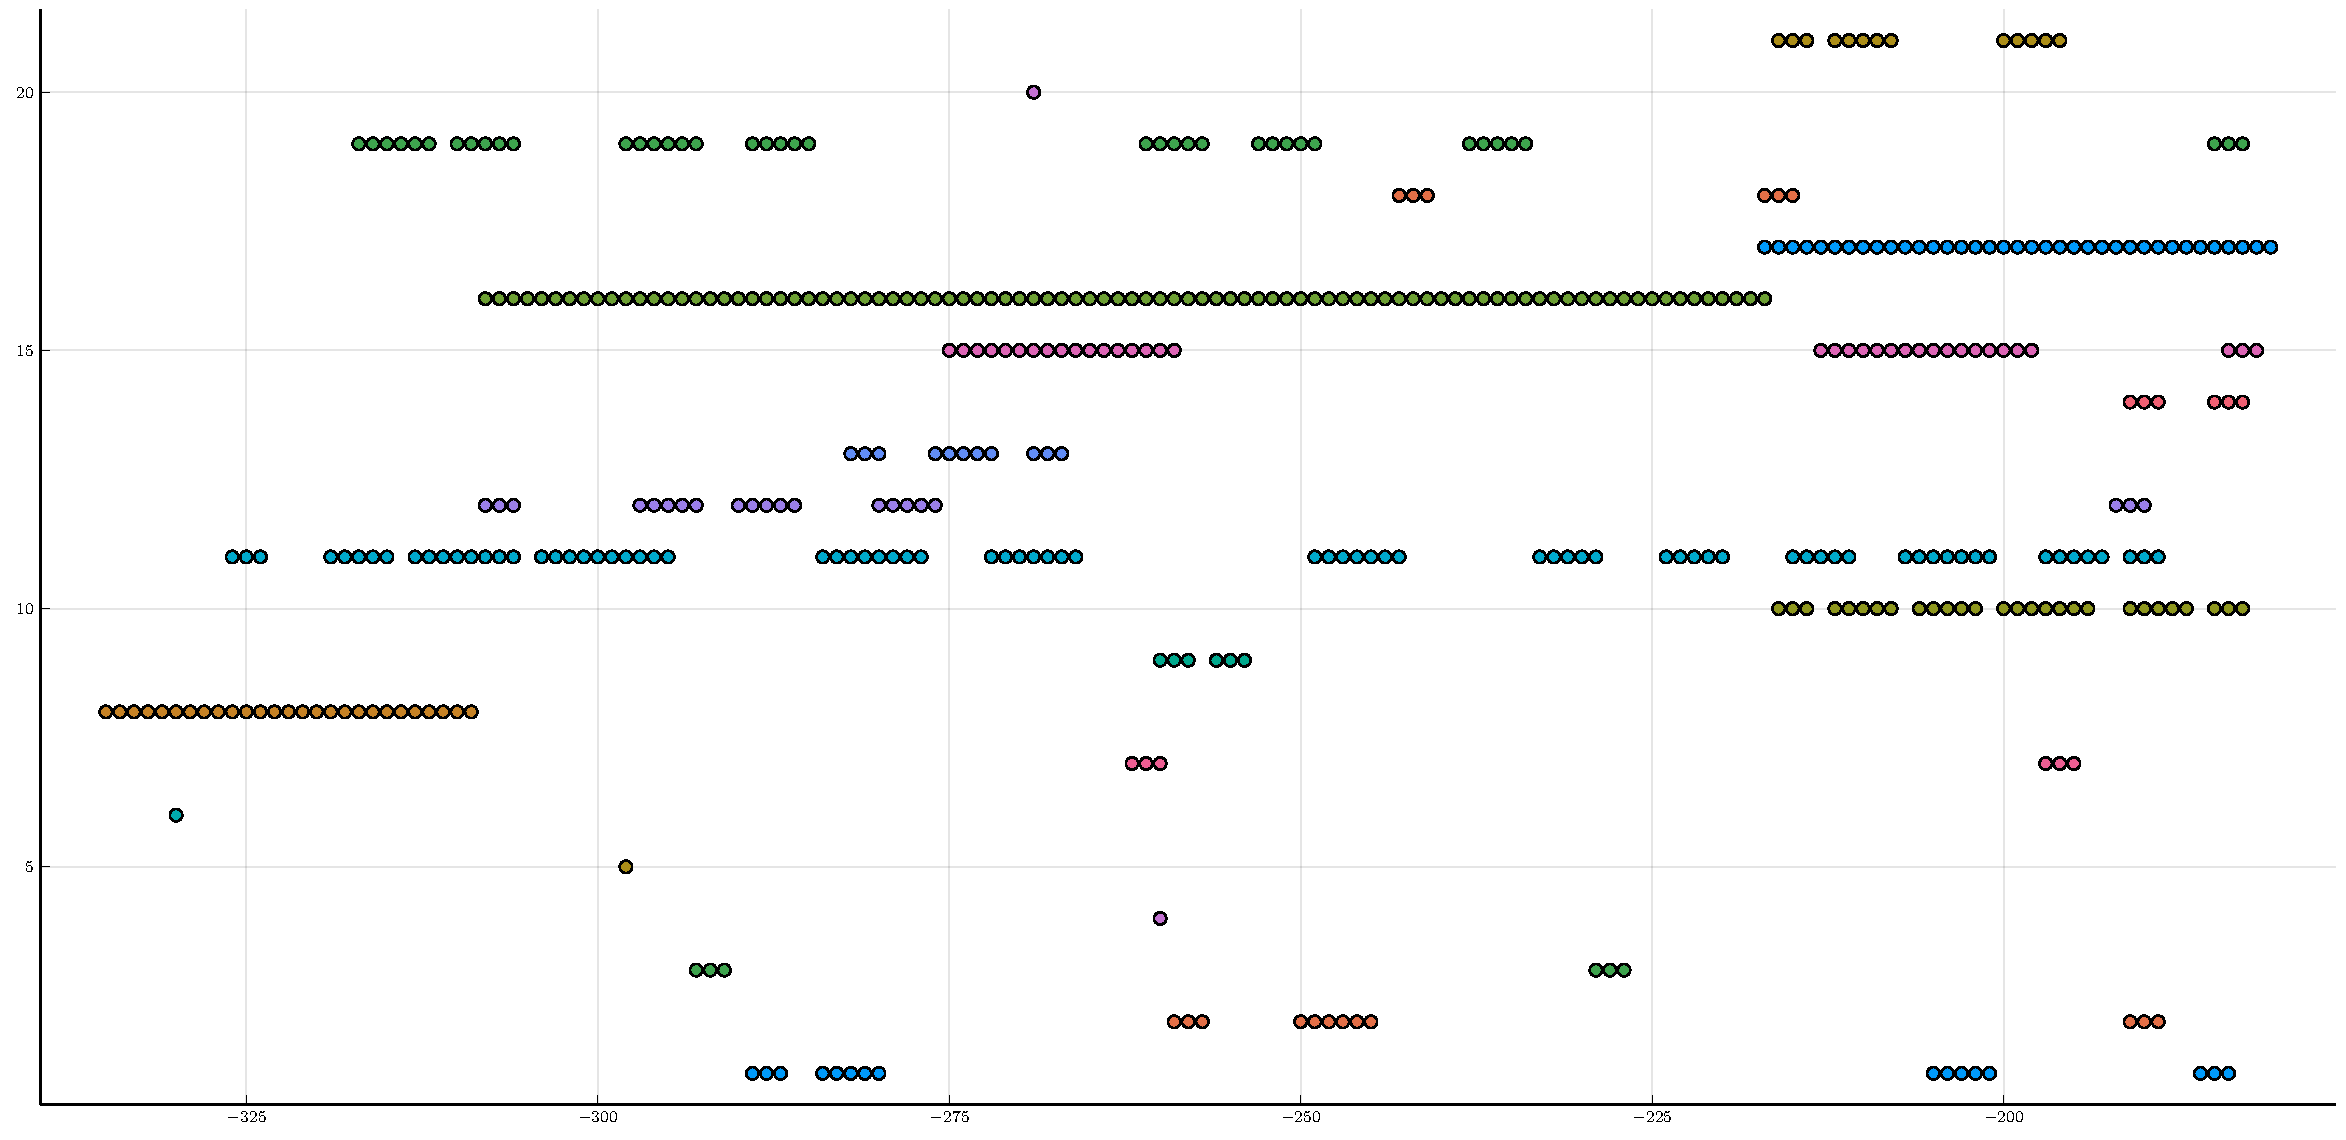
\includegraphics[width=\textwidth]{images/CZAC00-swflows-passivednshostname0/CZAC00-swflows-passivednshostname0.pdf}
		\caption{The CZAC00 hostname from pDNS over time}
	\end{figure}
\end{frame}

\begin{frame}{Let's introduce the method...}
	\begin{itemize}
		\item HARP - a method for pretraining on simplified graphs
		\item The simplified graphs are generated in the way depicted bellow
		\item The embedding is trained from the coarsest to the finest graph
	\end{itemize}
	\begin{figure}
		\centering
		\begin{subfigure}[t]{0.38\textwidth}
			\centering
			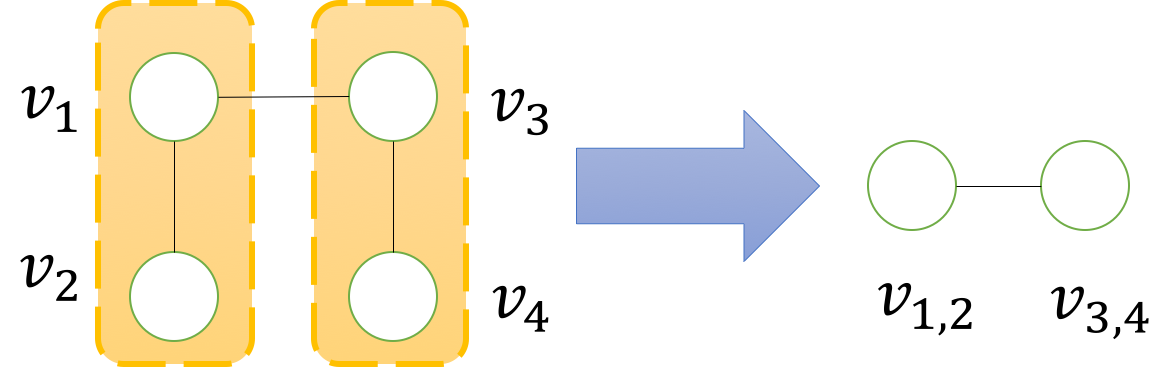
\includegraphics[width=\textwidth]{images/edge_collapsing.png}
			\caption{Edge collapsing}
		\end{subfigure}
		\hspace{2em}
		\begin{subfigure}[t]{0.38\textwidth}
			\centering
			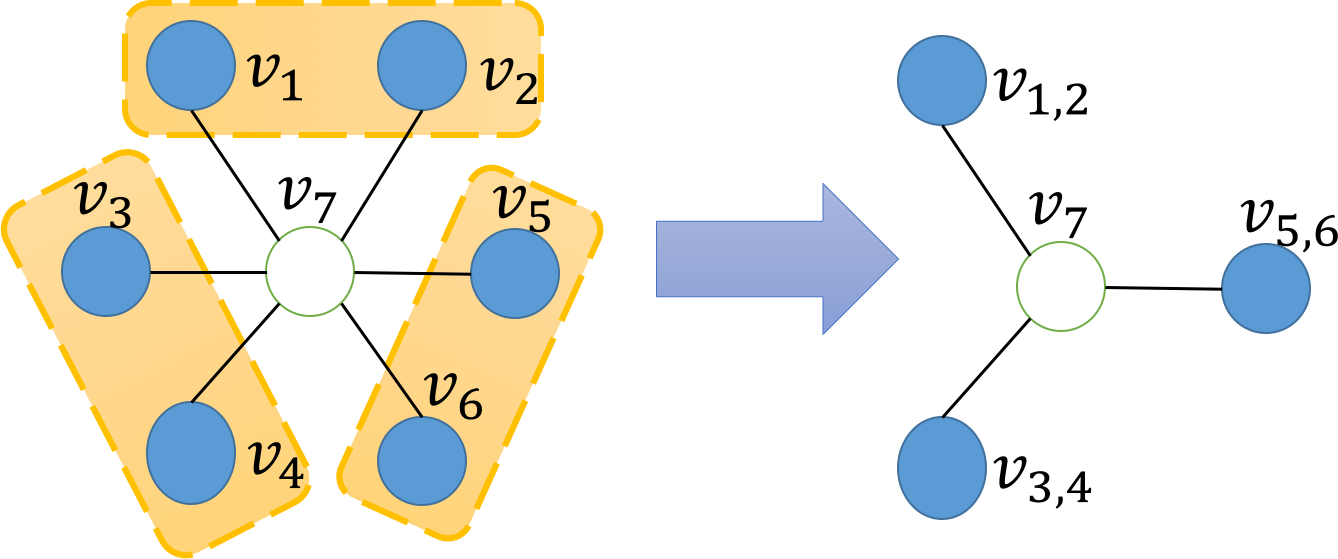
\includegraphics[width=\textwidth]{images/star_collapsing.png}
			\caption{Star collapsing}
		\end{subfigure}
	\end{figure}
\end{frame}

\begin{frame}{...and some theory behind it}
	\begin{itemize}
	  \item Graph homomorphisms (i. e. subgraph isomorphism)
\[ uv \in E \left( G \right) \implies \varphi \left( u \right) \varphi \left( v \right) \in E \left( H \right) \]
	  \item Injective graph homomorphisms (i. e. subgraph isomorphism)
\[ \forall u, v \in V \left( G \right) \quad \varphi \left( u \right) = \varphi \left( v \right) \implies u = v \]
	  \item Partially injective graph homomorphisms (i. e. subgraph isomorphism)
\[ \forall uv \in \mathcal{C} \quad \varphi \left( u \right) = \varphi \left( v \right) \implies u = v \]
	    where \( \mathcal{C} \subseteq \left( V \left( G \right) \right)^2 \setminus E \left( G \right) \)
	\end{itemize}
\end{frame}

\begin{frame}{How do these 2 relate?}
	\begin{itemize}
		\item We can express the HARP transformations as P. I. homomorphisms
		\item The set of all partially injective homomorphisms between 2 graphs forms a lattice, allowing for searching for the coarsening operation tailored to the problem at hand
		\item In this way, you can either preserve or collapse the substructure you are interested in
		\item In the future, the coarsening operation could be learned
	\end{itemize}
\end{frame}

\begin{frame}{Experimental verification of HARP based on PIHom}
	\begin{figure}
		\centering
		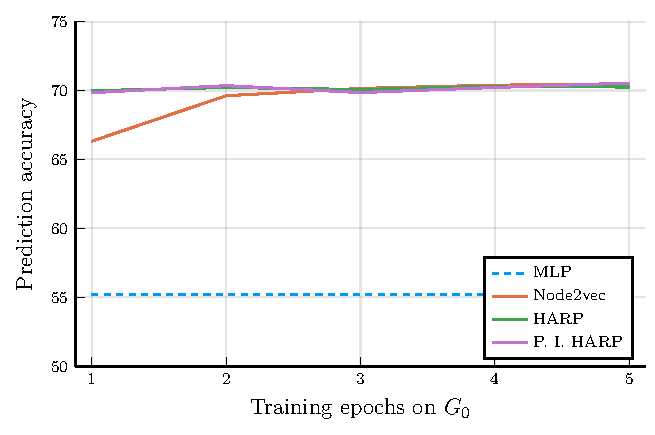
\includegraphics[width=0.8\textwidth]{images/pihom_comparison/pihom_comparison.pdf}
		\caption{Prediction accuracy on OGBN-arxiv}
	\end{figure}
\end{frame}

\begin{frame}{HARP as a complexity-performance trade-off}
	\begin{itemize}
		\item The fact that HARP trains on smaller graphs could be exploited for gains in computational complexity
		\item Experiment: How fast does node2vec train on a graph with and without HARP pretraining?
	\end{itemize}
\end{frame}

\begin{frame}{HARP as a complexity-performance trade-off}
	\begin{figure}
		\centering
		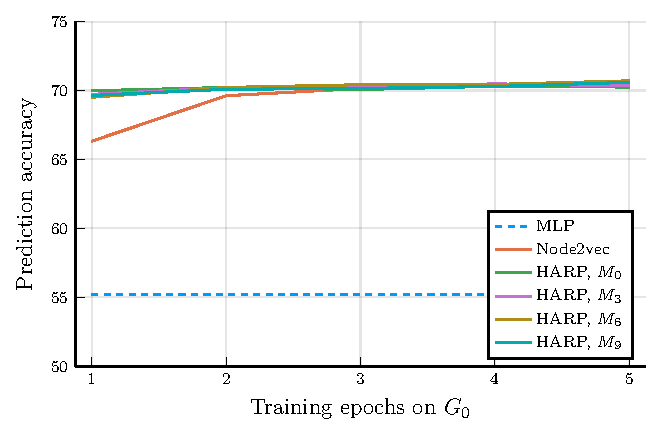
\includegraphics[width=0.8\textwidth]{images/steps_accur/steps_accur.pdf}
		\caption{Prediction accuracy on OGBN-arxiv}
	\end{figure}
\end{frame}

\begin{frame}
	\centering
	% TODO
\end{frame}

\end{document}
